\chapter{High Doping Concentrations in Nanowires}
\label{sec:high}

This chapter will discuss the concentration of dopants incorporated into ion irradiated nanowires. The simulations and experiments presented in this chapter where all performed with $175\, keV\,Mn^+$ irradiated $ZnO$ nanowires, however, the effects are easily applied to other material combinations. Some of the first results were published in reference \cite{johannes_enhanced_2014}.

\section{Doping and Sputtering}

With \emph{iradiana} the distribution of the places where the ions come to rest gives the profile of the concentration of dopants per fluence. Locally the concentration [$\nicefrac{atoms}{cm^{3}}$] increases a certain amount per fluence [$\nicefrac{ions}{cm^{2}}$], leading to the somewhat awkward unit of for the doping efficacy $[\nicefrac{(atoms/cm^{3})}{(ions/cm^{2})}]$. An example of the dopant distribution simulated with \emph{iradina} is shown in figure \ref{iradinacrossection}a for the irradiation of a $ZnO$ nanowire with $175\,keV\,Mn^+$. The ions enter the $y$-$z$ plane at random locations and at an angle of $45^\circ$ to the $z$-axis, which is periodically continued outside the plane of the image. It is clear that a homogeneous doping profile is not easy to obtain for the irradiation of a nanowire from one side. As with the creation of a box profile in bulk irradiation, multiple irradiation steps with varying energy are required. Note that an ion energy of $175\,keV$ is obviously not enough to permeate the whole nanowire diameter of $200\,nm$, so that an additional irradiation with higher ion energy would be required to obtain homogeneous doping. Rotating the nanowire under the ion beam is a much easier way of increasing homogeneity of the doping profile. Figure \ref{iradinacrossection}b shows the local dopant incorporation efficacy for the rotation of the profile show in \ref{iradinacrossection}a. Irradiation with a single, relatively low ion energy produces a homogeneous doping profile. 
  
\begin{figure}
	\centering
		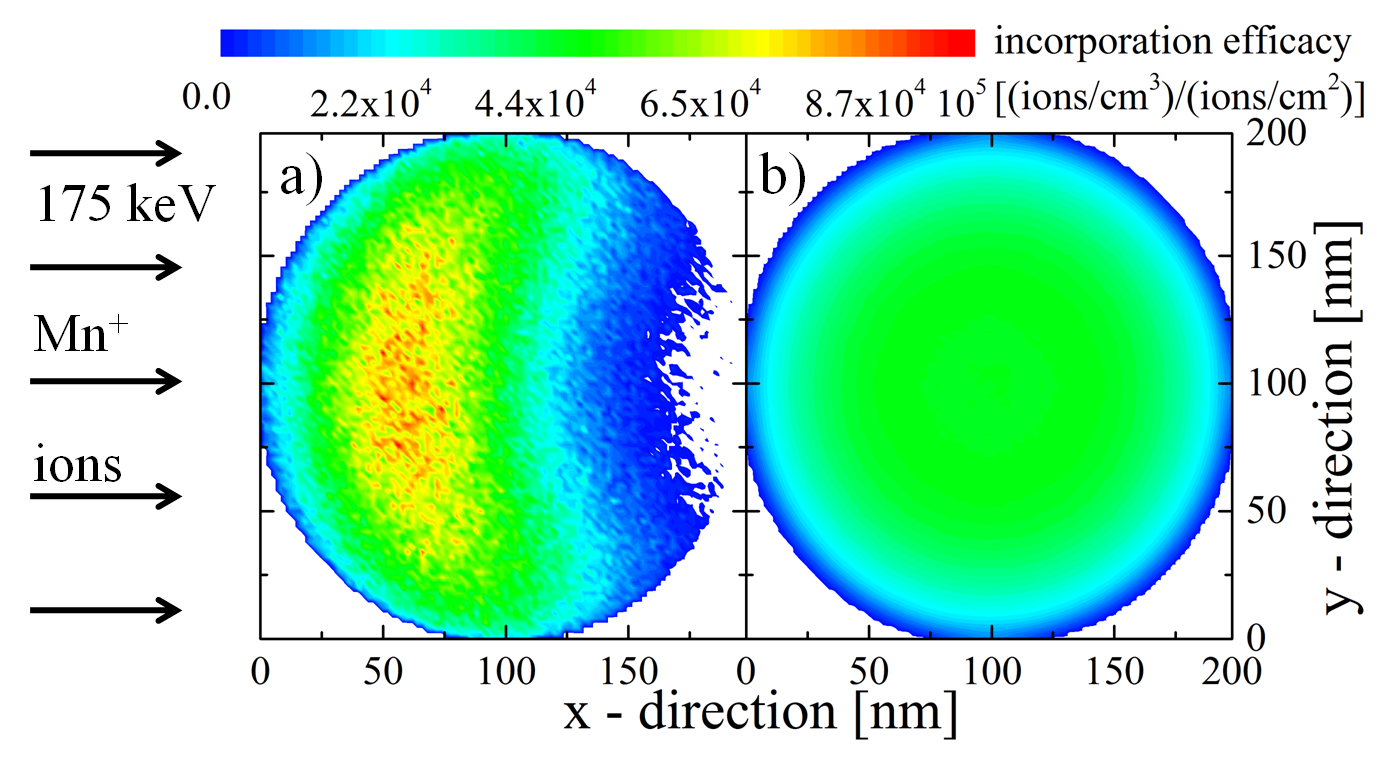
\includegraphics[width=.8\textwidth]{images/iradinacrosssection.png}
	\caption{a) Color plot of the increase in concentration per fluence for the irradiation of a $ZnO$ nanowire with $175\,keV\,Mn^+$ ions at an angle of $45^\circ$ to the $z$-axis. The energy was selected so that the rotation of this profile produces a radially homogeneous dopant distribution, as shown in b). The mean dopant incorporation efficacy is $3.6\cdot10^4\,\nicefrac{(atoms/cm^3)}{(ion/cm^2)}$.}
	\label{iradinacrossection}
\end{figure} 

As lower energy ions have lower ranges, there are fewer paths that cause the ion to leave the nanowire, particularly in the forward direction. Therefore, the first advantage of decreasing the ion energy is that the doping efficacy is larger for lower ion energies, so a lower irradiation fluence is required to achieve doping at a desired level. Furthermore, lower ion energy impacts also produce less damage in the irradiated matrix. Together with an optimal irradiation temperature, the rotated irradiation was utilized to improve the magnetic properties of $Mn^+$ irradiated $GaAs$ nanowires \cite{borschel_new_2011,paschoal_hopping_2012,borschel_ion-solid_2012,kumar_magnetic_2013,paschoal_magnetoresistance_2014}. 


%In figure \ref{iradinacrossection}b the outermost layer of the nanowire has a lower dopant incorporation efficacy than the rest of the wire volume. The sputtered atoms predominantly originate from this outer layer, so that the matrix of the nanowire is eroded preferentially to the incorporated dopants. 

\vfill
\section{nano-XRF on single nanowires}

The expected non-linear increase in doping concentration with the ion fluence was first investigated on $ZnO$ nanowire samples grown in Jena, such as the one shown in figure \ref{ZnOwires}a. The nanowires were transferred onto the carbon-foil of a $Cu$ TEM grid by imprinting after the rotated irradiation with $0.24, 0.48, 0.95$ and $1.9\cdot 10^{17}\,\nicefrac{ions}{cm^2}\,Mn^+$ ions at $175\,keV$; corresponding to $Mn/Zn$ ratios of $0.02, 0.04, 0.08$ and $0.16$, as extrapolated from the mean doping efficacy obtained from the \emph{iradina} simulation.

\begin{figure}[H]
	\centering
		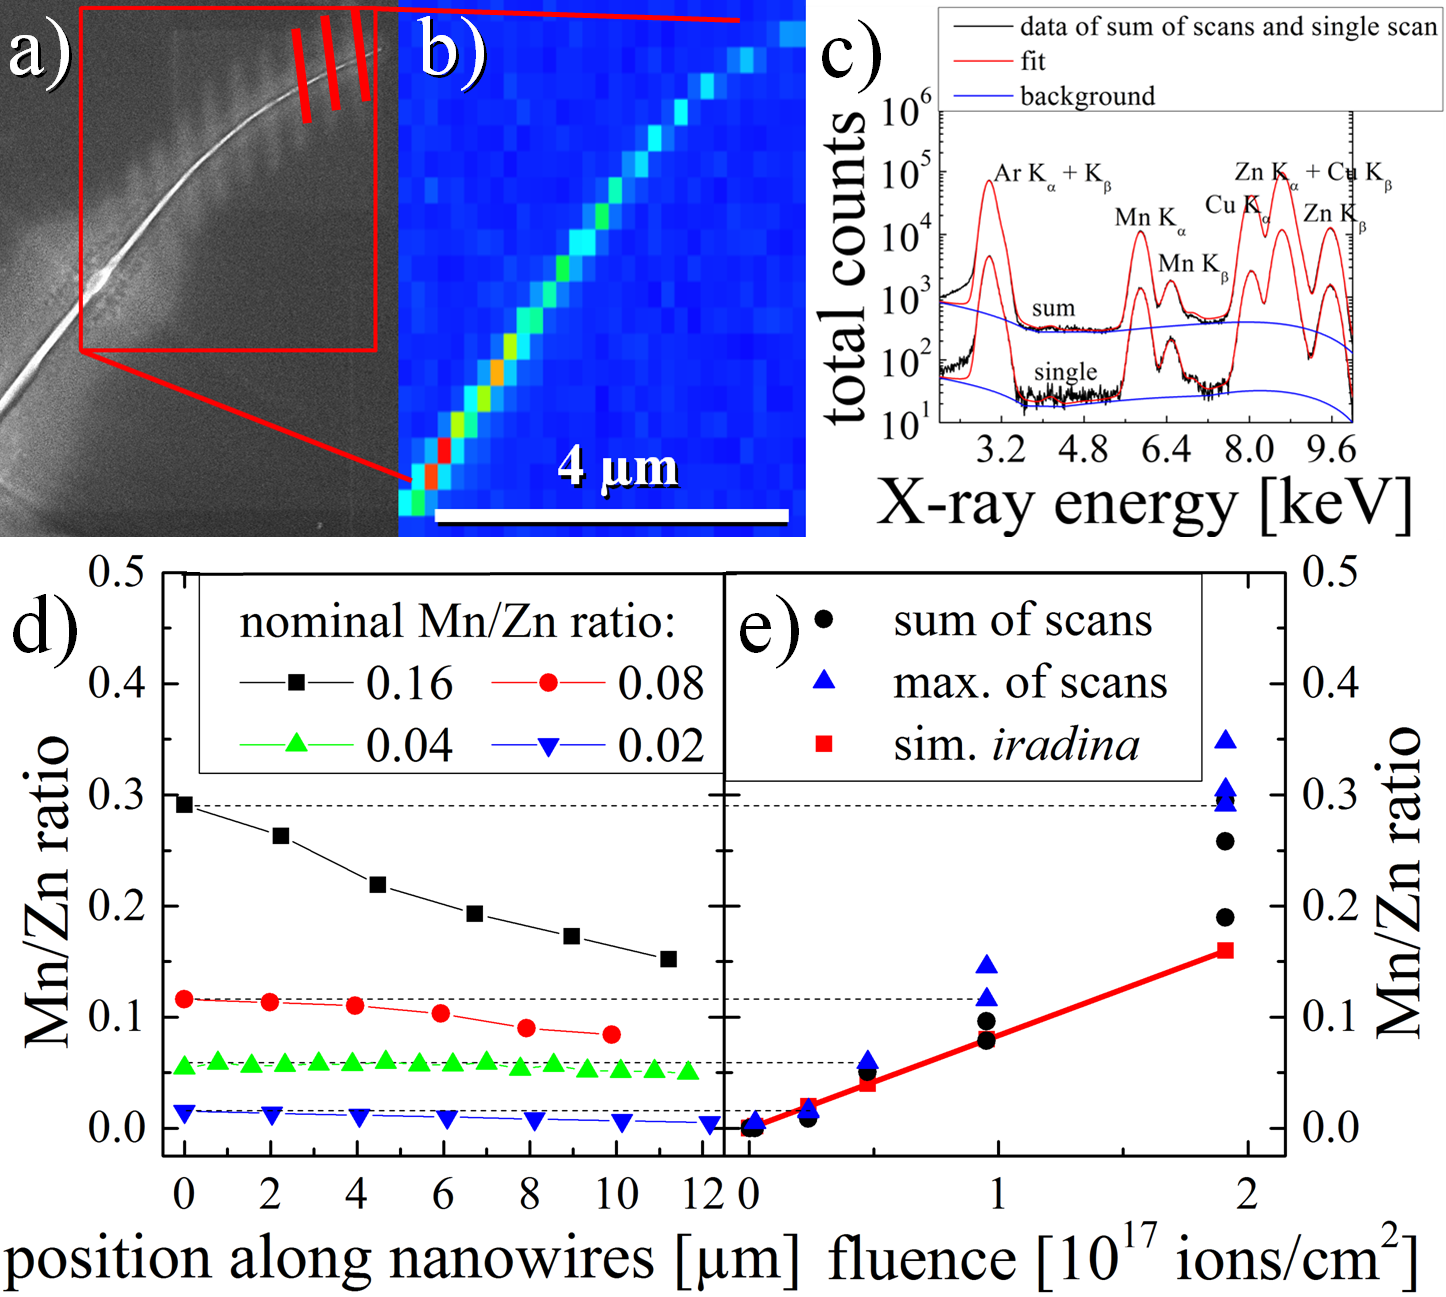
\includegraphics[width=.7\textwidth]{images/largeXRF.png}
	\caption{a) SEM image of a $175\,keV\,Mn^+$ irradiated $ZnO$ nanowire on the carbon-foil of a $Cu$ TEM grid after XRF investigation. The red lines indicate where the focused X-ray beam was scanned with a long integration time. b) Intensity map of the X-ray signal. c) Exemplary XRF-spectra of a single scanned line and for the sum of all the lines for the nanowire shown in a) and b). d) $Mn/Zn$ ratio quantified with PyMCA for representative wires along the length of the nanowires for varying nominal concentrations. The corresponding data points in the plot of the concentration versus the irradiated ion fluence in e) are connected with a dashed line. The red data points and line in e) indicate the linear extrapolation to the nominal $Mn/Zn$ ratio from \emph{iradina} simulations. The black circles show the average ratio obtained by fitting to the sum of all scans, while the blue upturned triangles show the maximum ratio found for along the length of a nanowire.} 
	\label{largeXRF}
\end{figure} 

Figure \ref{largeXRF}a shows a SEM image of one of the $Mn^+$ irradiated $ZnO$ nanowires investigated by nano-XRF at the ESRF. At one point the nanowire shows some damage where the exposure to the XRF-beam was prolonged during the navigation on the sample. Also the track of the intense, focused X-ray beam can be seen on the carbon foil by some redeposition of material. All in all, the damage to the nanowire is, however, not large enough to have an effect on the quantification, especially considering that this particular nanowire was selected as it showed the most pronounced effects. In \ref{largeXRF}b a map of the detected X-ray intensity clearly shows the nanowire. The XRF spectrum collected for one of the scans indicated in the SEM image \ref{largeXRF}a is shown in \ref{largeXRF}c. The number of counts for a single scan is comfortably sufficient to quantify the $Mn$ and $Zn$ content. The average concentration for a nanowire was determined by fitting the sum XRF-spectrum of all scans across the nanowire. The $Mn/Zn$ ratio is plotted over the position along the nanowire for the four nominal concentrations in figure \ref{largeXRF}d. Clearly there is a significant gradient in the $Mn$ concentration along the nanowire length. The maximum $Mn/Zn$ ratio was always found at the tip of the nanowire, which was identifiable in the SEM images by the slight tapering of the nanowires. The $Mn/Zn$ ratio for both the sum of all scans, as well as the scan at the tip showing the maximum $Mn/Zn$ ratio is plotted in \ref{largeXRF}e alongside the nominal ratio extrapolated from \emph{iradina} simulations.
  
Two pieces of information can be gained from these results. First, the nanowires on the sample clearly shadowed each other from the ion beam, leading to the pronounced $Mn$ concentration gradient. The shadowing is least at the tips of the nanowires, therefore the corresponding data points are the closest to the simulated situation. This emphasizes the second point, that the increase in $Mn$ concentration with the ion fluence is much stronger than the linear extrapolation from static simulations. The assumption underlying the doping efficacy gained from the earlier simulations and using it to calculate the required fluence for a desired doping concentration is that the concentration increases linearly with the irradiated fluence. However, this is only true in the absence of sputtering. Sputtering erodes the target nanowire at the same time as ions are incorporated. It thus leads to a non-linear increase in the concentration of dopants with the irradiated fluence. To separate these two effects the irradiation and quantification has to be repeated with nanowires with a sparser lateral distribution, as shown in \ref{ZnOwires}b. These were kindly provided by Dr. Helena Franke from the University Leipzig.

\begin{figure}
	\centering
		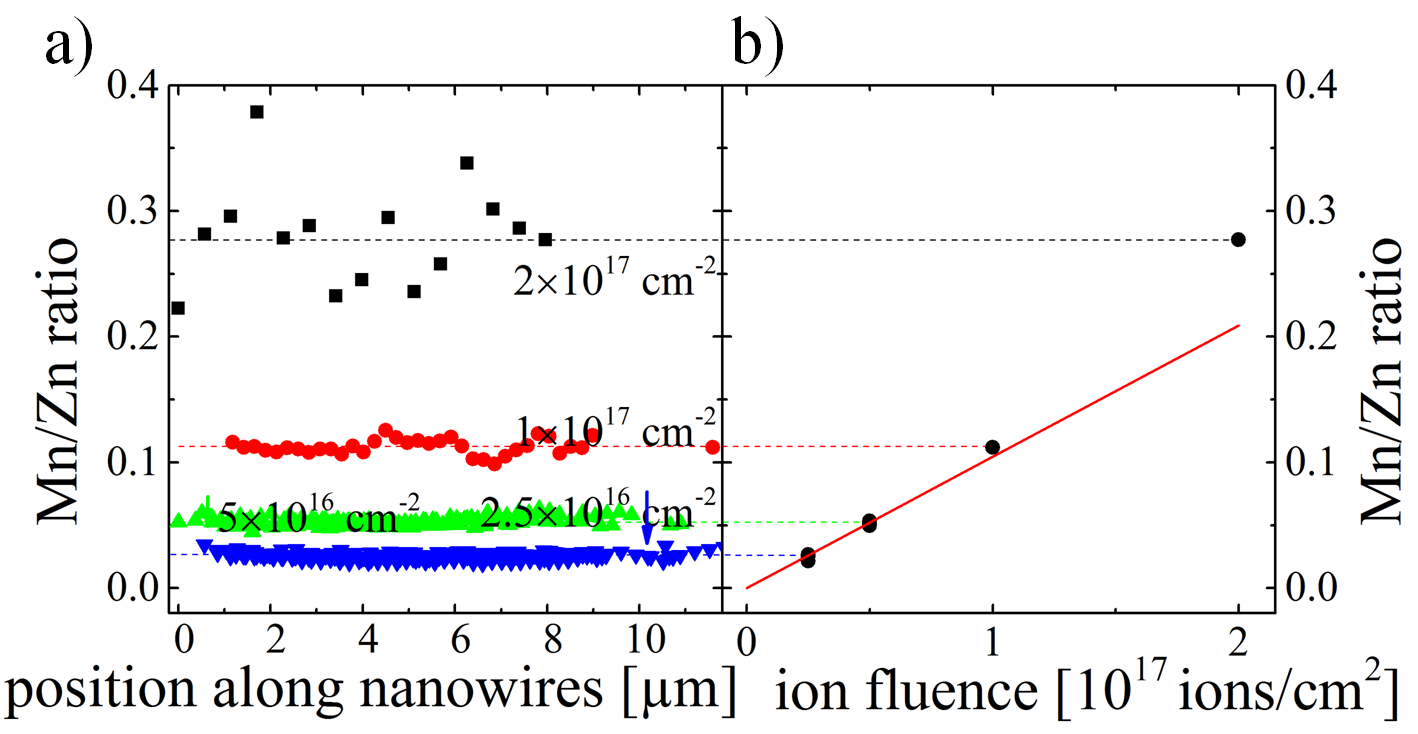
\includegraphics[width=.85\textwidth]{images/MnZn2.png}
	\caption{a) $Mn/Zn$ ratio along the wire length for sparse nanowire samples irradiated with the indicated ion fluence of $175\,keV Mn^+$. There is no concentration profile along the wire length. In b) the black circles show the average ratio obtained by fitting to the sum of all scans for the respective ion fluence. The red line in b) shows the linear extrapolation from \emph{iradina} simulations. }
	\label{MnZn2}
\end{figure} 

The same experimental procedure was followed to investigate the Mn/Zn ratio with the sparser nanowire samples, only rounding the rotated irradiation fluence to $0.25, 0.5, 1$ and $2\cdot 10^{17}\,\nicefrac{ions}{cm^2}\,Mn^+$. The results from the nano-XRF quantification of these nanowires is shown in figure \ref{MnZn2}. The $Mn/Zn$ ratio plotted against the nanowire length in \ref{MnZn2}a no longer shows any gradient. As these wires were individually transferred to the lacy carbon TEM grid, they could be investigated by SEM before and after irradiation. The diameter of the nanowire irradiated with the highest fluence was reduced from $202\,nm$ to $93\,nm$ by sputtering, while the lower fluences produced lower reductions in diameter, as expected. From these diameter reductions the sputter yield can again be calculated, yielding values in the range of 5 - 20. As seen in the dedicated study on sputtering these values have a very large spread. Also the $Mn/Zn$ ratio for the nanowires irradiated with higher fluences shows a significant spread due to the fact that the thinned nanowires have a much smaller volume and thus give a lower XRF signal. Added to this, the thinner wires could only be attached to the lacy carbon loosely, so that they drifted much more during the XRF scans making it impossible to increase the integration time significantly to compensate for the lower signal. Nevertheless, the average $Mn/Zn$ ratio is accurate to within $\pm\,0.01$, as it is based on the sum of all spectra including a sufficiently large number of counts. The average values for all irradiated fluences is plotted in \ref{MnZn2}b against the irradiated fluence. As with the denser nanowire sample, again the increase in the $Mn$ concentration is much larger and non-linear than the simple linear extrapolation from the \emph{iradina} simulation. Now we can be sure that the incorporation is not effected by the shadowing of the nanowires amongst themselves.


\section{Pseudo-dynamic simulation}

The direct simulation of the effect of sputtering on the incorporation of dopants into nanowires requires a dynamic simulation program, which also considers the three dimensional geometry of the target. As such software is not currently openly available, a step-by-step investigation using results from static simulations will be undertaken to discuss the observed interaction between dopant incorporation and sputtering.

\begin{SCfigure}
	\centering
		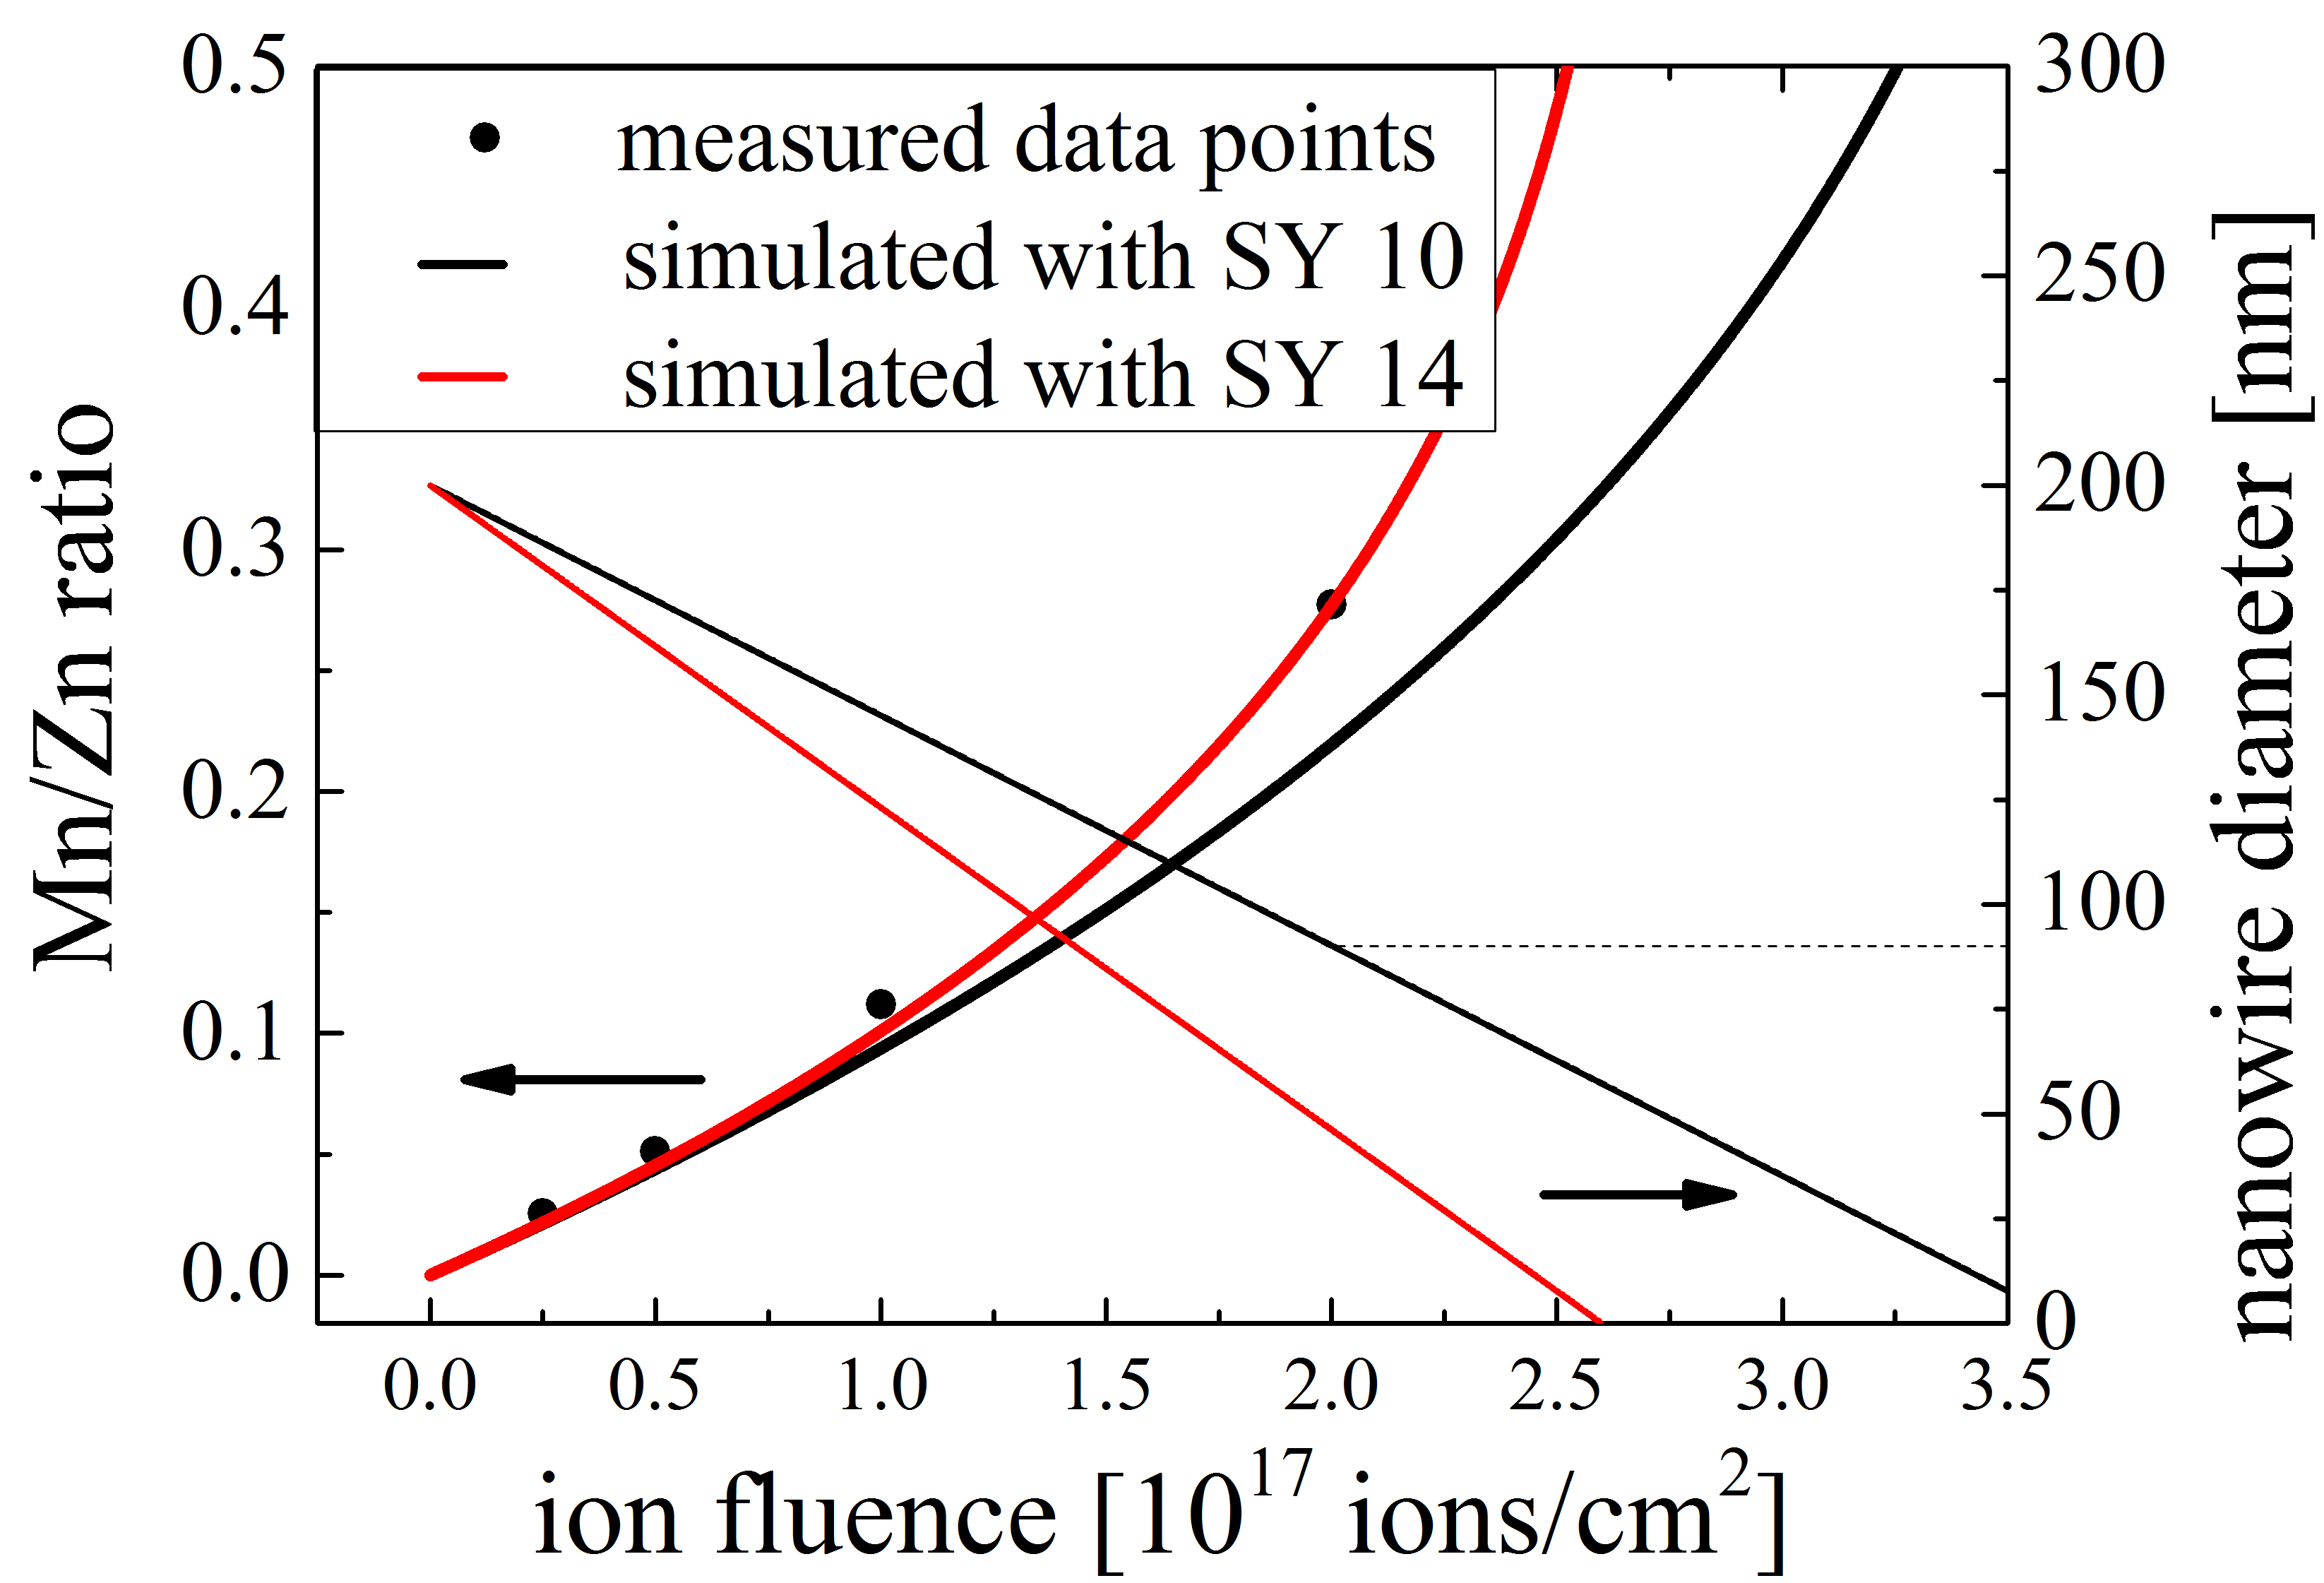
\includegraphics[width=.5\textwidth]{images/staticsputteryield.png}
	\caption{Plot of the $Mn/Zn$ ratio (left axis) versus the irradiated ion fluence of $175\,keV Mn^+$ for the measured nanowires and two simulations, indicated by black circles, a black line and a red line respectively. The nanowire diameter (right axis) is also plotted against the fluence for both simulations. The dashed line at $90\,nm$ marks the final radius of the data point corresponding to the highest irradiated fluence.}
	\label{staticsputter}
\end{SCfigure} 

The most straightforward approach is to consider the total sputter yield and the doping efficacy constant. With these assumptions and a reiterative calculation of incremental fluence steps, a pseudo-dynamic simulation can be numerically constructed. The $Mn$ concentration increases with each irradiated fluence step by the value determined by the doping efficacy. Then the number of $Zn, O$ and $Mn$ atoms is reduced by sputtering so that the total sputter yield is divided between $Zn+O$ and $Mn$ according to the current $Mn$ concentration. The total number of atoms is used to calculate the new nanowire radius and the next incremental fluence step can be calculated. Figure \ref{staticsputter} shows the experimentally determined $Mn/Zn$ ratios next to such a simulation. The doping efficacy was set to the same value used for the linear extrapolation so far, $3.6\cdot10^4\,\nicefrac{(atoms/cm^3)}{(ion/cm^2)}$. The total sputter yield was set to 10 for the simulation yielding the values depicted in black. This value corresponds to the sputter yield determined from the reduction in the radius of the nanowire irradiated with $2\cdot10^{17}\,\nicefrac{ions}{cm^2}$ and therefore, unsurprisingly, this simulation produces the the correct diameter of $\approx\,90\,nm$ at this ion fluence. However the calculated $Mn/Zn$ ratio is too low. Conversely, a simulation with a larger sputter yield of 14, indicated in red, correctly reproduces the $Mn/Zn$ ratio, but erodes the nanowire too quickly. Nevertheless, the overall agreement between the experiment and the simulation seems promising.

To increase the accuracy of the pseudo-dynamic simulation, results from a set of static simulations for varying diameters can be used. The sputter yield is dependent on the nanowire radius and the ion energy as shown in \ref{sputterincorporate}a. This relation is discussed in detail in the previous chapter \ref{sec:simsputering}. Likewise the incorporation efficacy plotted in \ref{sputterincorporate}b is also dependent on the nanowire radius and the ion energy. For a fixed diameter and increasing ion energy the efficacy is monotonically decreasing, as the probability of the ion to leave the nanostructure rises together with the ion range. For fixed ion energies, the probability of an ion to stay in the nanostructure increases with increasing diameter, so that at first the efficacy also increases with increasing diameter. For large diameters this effect is overcompensated by a stronger dilution of the dopants in the volume of the nanowire which increases as the square of the diameter. This leads to a maximum in the incorporation efficacy at diameters around twice the ion range. Note that the color scale in \ref{sputterincorporate}b is logarithmic.

\begin{figure}
	\centering
		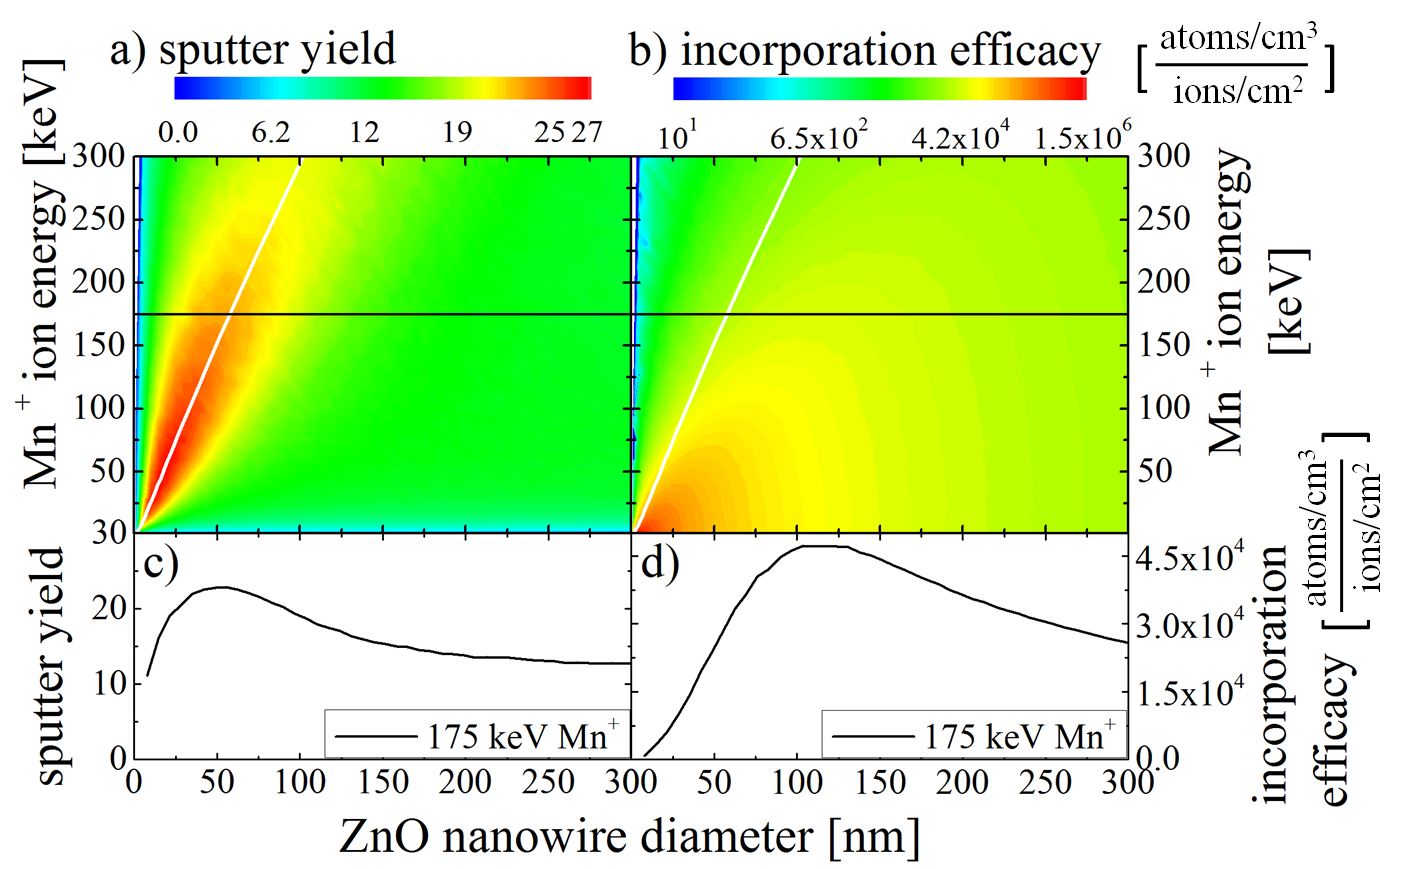
\includegraphics[width=.85\textwidth]{images/sputterincorporate.png}
	\caption{a) Sputter yield for the irradiation with $Mn^+$ of ZnO nanowires with varying diameters an ion energies. From the same simulations the dopant incorporation efficacy was determined and plotted in b). The white line in both plots indicates the ion range at the respective energy and $45^\circ$, calculated with SRIM for $Mn^+$ in $ZnO$. The horizontal black line indicates the energy used in the experiments and simulations in this chapter.}
	\label{sputterincorporate}
\end{figure} 

The numerical, pseudo-dynamic simulation can easily be adapted to use the diameter dependent values for the sputter yield and the dopant incorporation efficacy. The resulting $Mn/Zn$ ratios from such an simulation are plotted in figure \ref{pseudodynamic} as red squares. The stronger than linear increase in the $Mn/Zn$ ratio seems less pronounced in this simulation when compared to the simulation only considering constant sputtering and doping efficacy, as the doping efficacy starts decreasing markedly with decreasing diameter from diameters around $100\,nm$. Here, also the sputtering starts to increase as the ions start to reach the back of the now thinned nanowire. In the evolution of the diameter with the irradiated ion fluence, plotted in figure \ref{pseudodynamic} as a red line, the increased sputtering is noticeable as a slight increase in the slope of the curve at $2\cdot 10^{17}\,\nicefrac{ions}{cm^2}$.

\begin{SCfigure}[50][h]
	\centering
		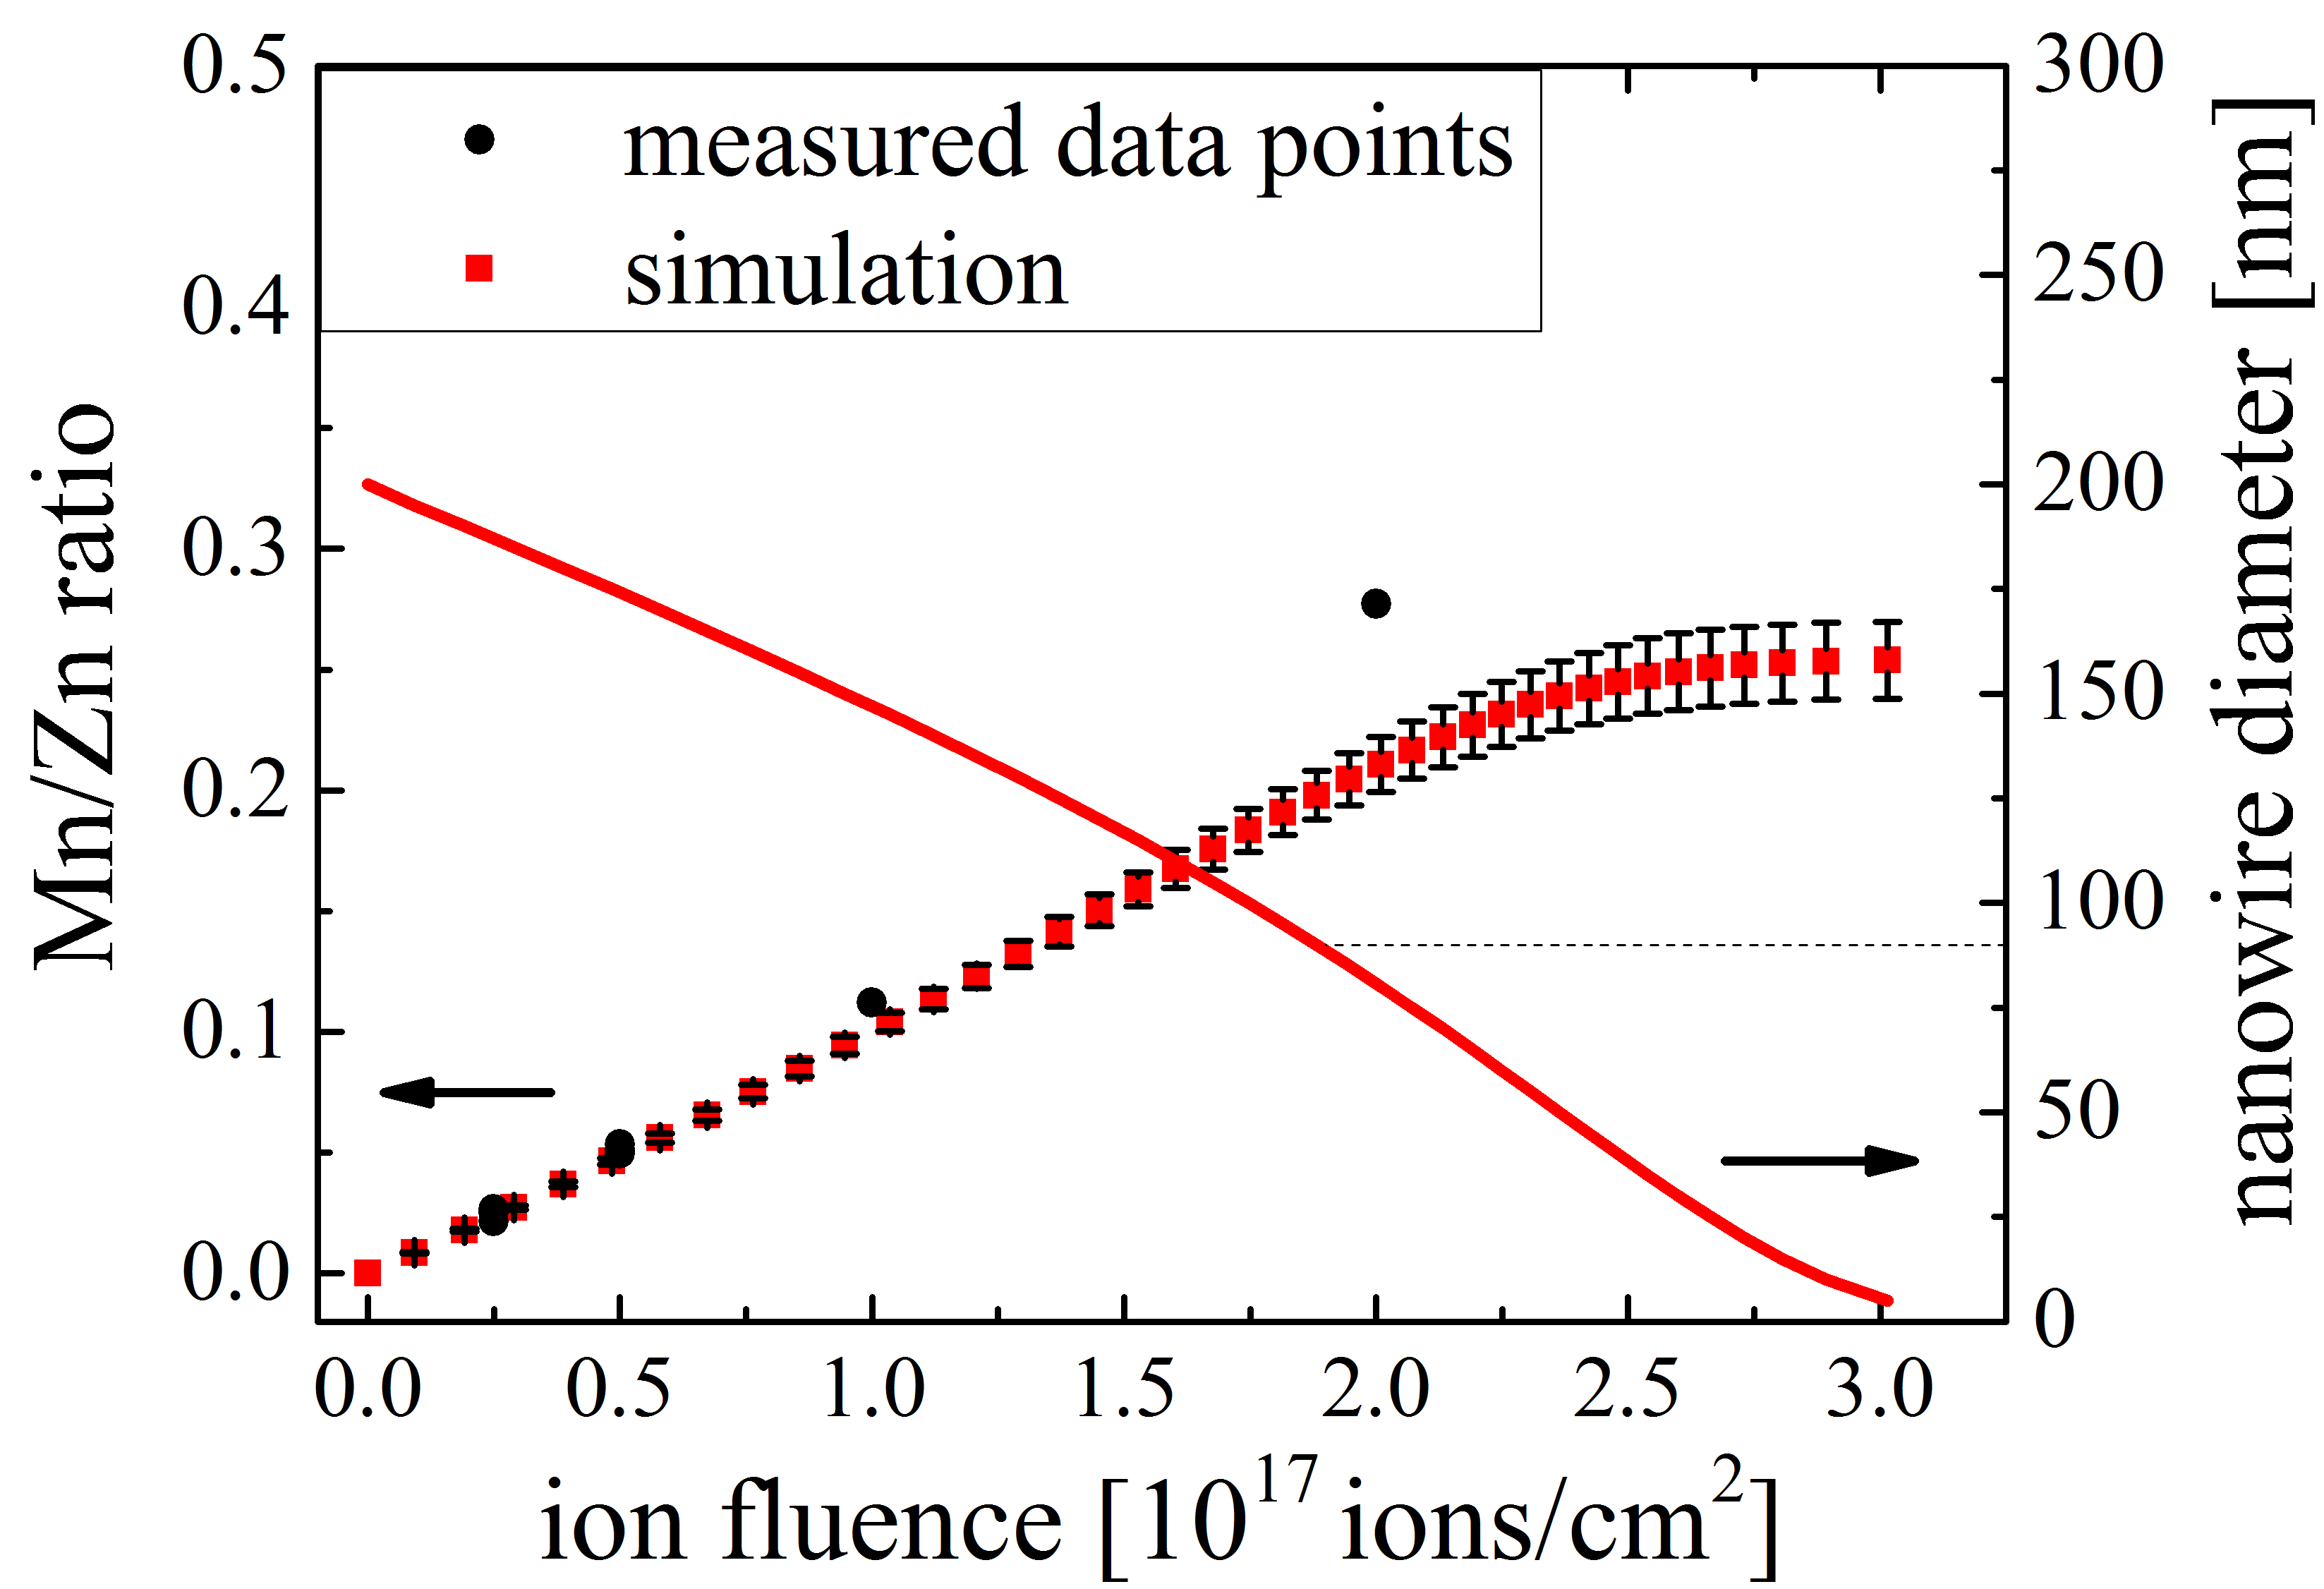
\includegraphics[width=.5\textwidth]{images/pseudodynamic.png}
	\caption{Results from a pseudo-dynamic simulation considering diameter dependent sputtering and doping efficacy. The $Mn/Zn$ ratio is plotted to the left axis versus the ion fluence of $175\,keV Mn^+$ as red squares for the simulation and black circles for the experiment. The error bars range from the $Mn/Zn$ ratio for $170\,keV$ to $180\,keV Mn^+$. The red line indicates the simulated nanowire diameter.}
	\label{pseudodynamic}
\end{SCfigure} 

\section{Discussion of relevant effects}

\subsubsection{Summarizing Discussion}